\documentclass{beamer}

\usepackage{comment}
\usepackage{color}
\usepackage{listings}
\usepackage{verbatim}
\usepackage{multicol}
\usepackage{booktabs}
\definecolor{green}{RGB}{0,128,0}

\newcommand\gehcomment[1]{{{\color{orange} #1}}}
\newcommand\add[1]{{{\color{blue} #1}}}
\newcommand\remove[1]{\sout{{\color{red} #1}}}
\newcommand\codecomment[1]{{{\color{green} #1}}}
\newcommand\redcomment[1]{{{\color{red} #1}}}
\newcommand\bluecomment[1]{{{\color{blue} #1}}}
\newcommand\greencomment[1]{{{\color{green} #1}}}
\newcommand\magentacomment[1]{{{\color{magenta} #1}}}

\begin{comment}
\tiny
\scriptsize
\footnotesize
\small
\normalsize
\large
\Large
\LARGE
\huge
\Huge
\end{comment}

\begin{document}
\title{Multiphase - Gas Injection}
\author{Emily Stein}
\date{\today}

%\frame{\titlepage}

%-----------------------------------------------------------------------------
\section{Description of Gas Injection}

\subsection{Gas Injection Conceptual Model}

\begin{frame}\frametitle{Description of Gas Injection Scenario}
The ``Gas Injection Scenario'' demonstrates how to set up a multiphase flow simulation using GENERAL MODE. It simulates gas injection into a 2D liquid saturated domain. Assumptions include:
\begin{itemize}
  \item Problem domain: $100 \times 1 \times 100$ m (x $\times$ y $\times$ z)
  \item Grid resolution: $5 \times 1 \times 5$ m 
  \item Flow mode: General
  \item Gas Source: Rate scaled by cell volume
  \item Maximum time step size: changes with simulation time
  \item Total simulation time: 100 y
\end{itemize}

\end{frame}

%-----------------------------------------------------------------------------
\frame{\frametitle{2D Gas Injection Scenario Schematic}
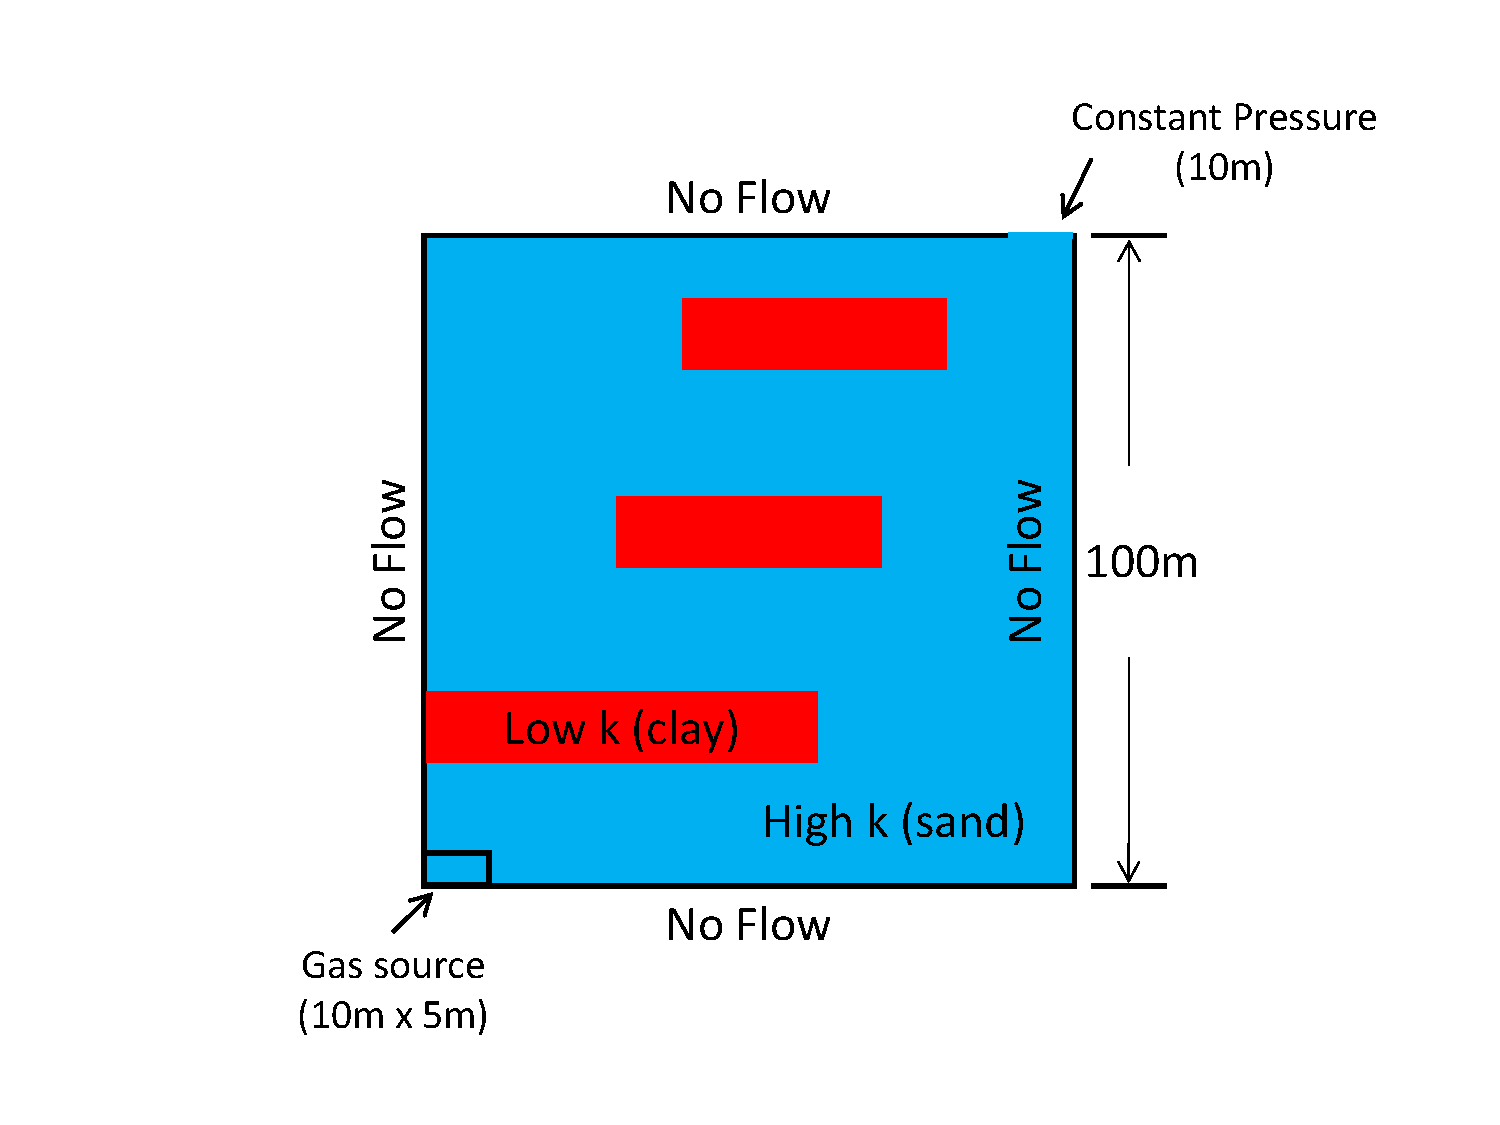
\includegraphics[width=\linewidth]{./gas_injection_bc}
}

%-----------------------------------------------------------------------------
\frame{\frametitle{2D Gas Injection Initial Conditions}
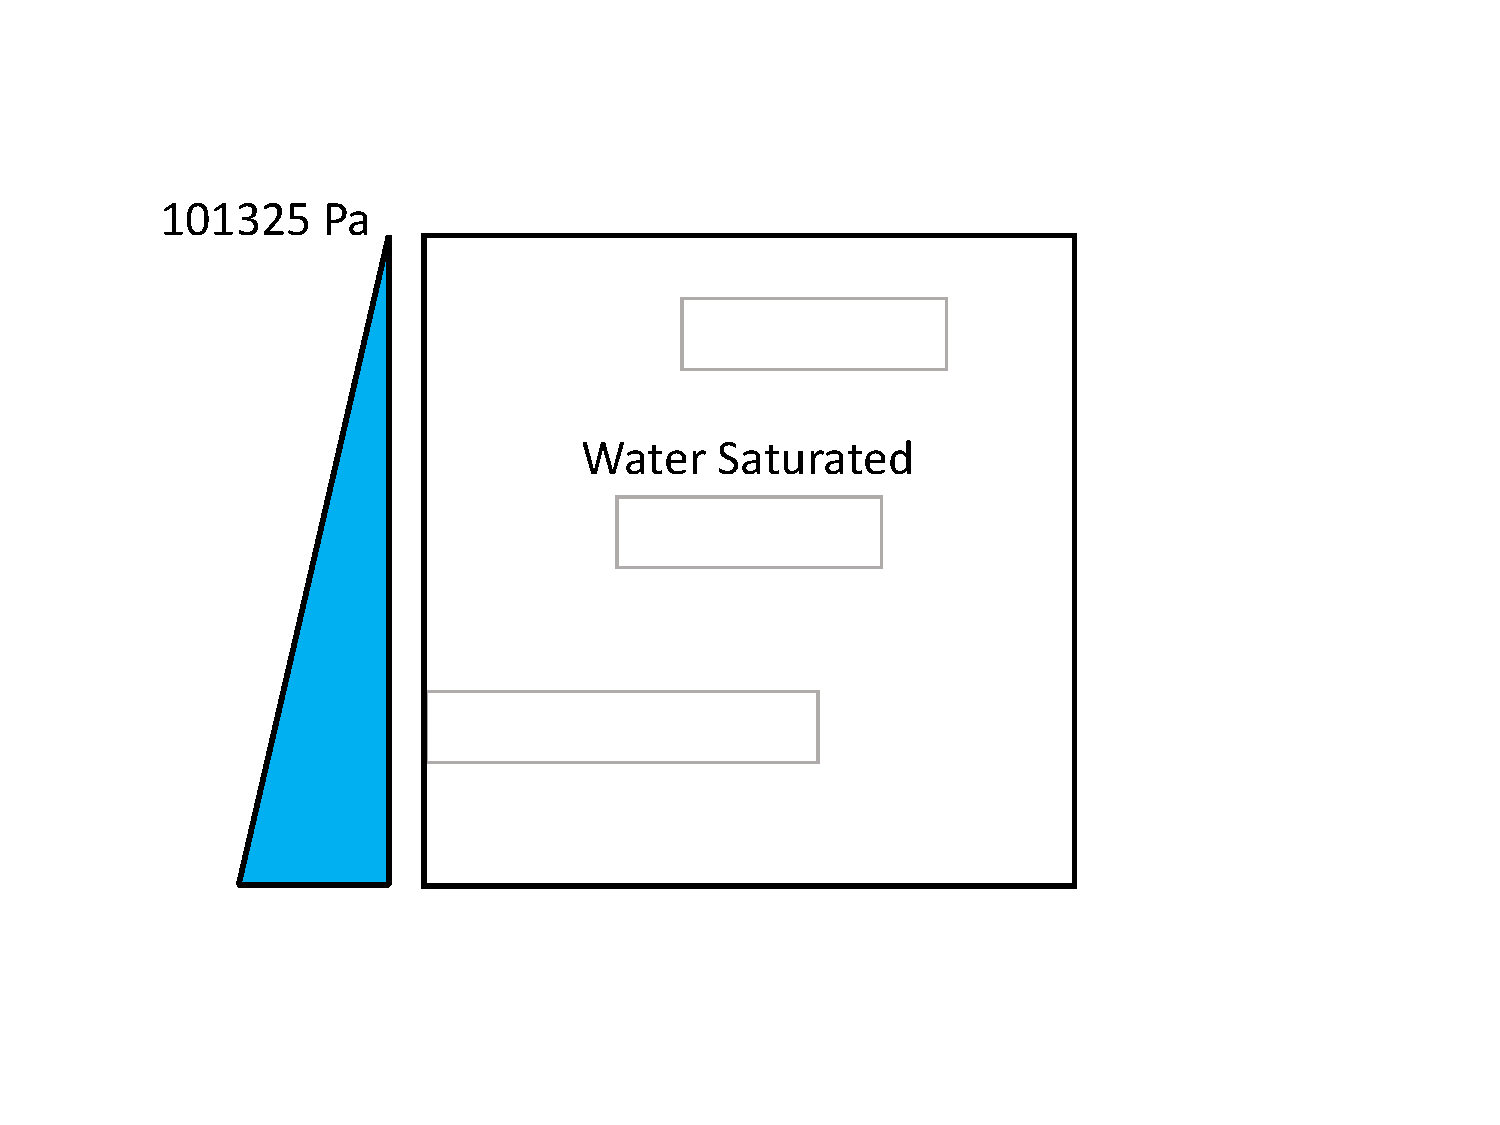
\includegraphics[width=\linewidth]{./gas_injection_ic}
}

%-----------------------------------------------------------------------------
\section{Description of Input Deck}

%-----------------------------------------------------------------------------
\subsection{SIMULATION}

\begin{frame}[fragile]\frametitle{SIMULATION}

\begin{itemize}
  \item Multiphase flow (General mode)
  \item with options
\end{itemize}

\begin{semiverbatim}\small
SIMULATION
  SIMULATION_TYPE SUBSURFACE
  PROCESS_MODELS
    SUBSURFACE_FLOW flow
      MODE GENERAL \bluecomment{! two-phase flow and energy}
      OPTIONS
        GAS_COMPONENT_FORMULA_WEIGHT 44.d0 \bluecomment{! CO2(g)} 
        ISOTHERMAL \bluecomment{! ignore energy component}
      /   
    /   
  /
END

SUBSURFACE
...
END_SUBSURFACE
\end{semiverbatim}

\end{frame}

%-----------------------------------------------------------------------------
\subsection{GRID}

\begin{frame}[fragile]\frametitle{GRID}

\begin{itemize}
  \item Problem domain: $100 \times 1 \times 100$ m (x $\times$ y $\times$ z)
  \item Grid resolution: $5 \times 1 \times 5$ m
\end{itemize}

\begin{semiverbatim}
GRID
  TYPE STRUCTURED
  NXYZ 20 1 20
  BOUNDS
    0.d0 0.d0 0.d0 \bluecomment{! xmin ymin zmin}
    100.d0 1.d0 100.d0 \bluecomment{! xmax ymax zmax}
  /
END
\end{semiverbatim}

\end{frame}

%-----------------------------------------------------------------------------
\subsection{FLUID\_PROPERTY}

\begin{frame}[fragile]\frametitle{FLUID\_PROPERTY}
\begin{itemize}
  \item Diffusion of dissolved gas in water
  \item Diffusion of water vapor in gas
\end{itemize}

\begin{semiverbatim}

FLUID_PROPERTY
  PHASE LIQUID \bluecomment{! for diffusion of dissolved gas}
  DIFFUSION_COEFFICIENT 1.d-9
END

FLUID_PROPERTY
  PHASE GAS \bluecomment{! for diffusion of water vapor}
  DIFFUSION_COEFFICIENT 2.1d-5
END
\end{semiverbatim}

\end{frame}

%-----------------------------------------------------------------------------
\subsection{OUTPUT}

\begin{frame}[fragile]\frametitle{OUTPUT}
\begin{itemize}
  \item Print a snapshot of entire solution periodically
  \item Print the solution at observation points every time step
  \item Print mass balance file every time step
  \item Choose output variables
\end{itemize}

\end{frame}

\begin{frame}[fragile]\frametitle{OUTPUT}

\begin{semiverbatim}\small
OUTPUT
  SNAPSHOT_FILE
    FORMAT HDF5
    PERIODIC TIME 0.01 y between 0. y and .1 y \bluecomment{! every 0.01 y}
    PERIODIC TIME 0.1 y between 0. y and 5. y  \bluecomment{! then 0.1 y}
    PERIODIC TIME 1. y between 0. y and 30. y  \bluecomment{! etc.}
    PERIODIC TIME 10. y between 0. y and 100. y
  /
  OBSERVATION_FILE
    PERIODIC TIMESTEP 1 \bluecomment{! print every time step}
  /
  MASS_BALANCE_FILE
    PERIODIC TIMESTEP 1 \bluecomment{! print every time step}
  /
  VELOCITY_AT_CENTER \bluecomment{! of cell}
  VARIABLES
    LIQUID_SATURATION
    GAS_SATURATION \bluecomment{! see input deck for more}
  /
END
\end{semiverbatim}

\end{frame}

%-----------------------------------------------------------------------------
\subsection{TIME}

\begin{frame}[fragile]\frametitle{TIME}
\begin{itemize}
  \item Final simulation time = 100 y
  \item Maximum time step size = 5 y
\end{itemize}

\begin{semiverbatim}

TIME
  FINAL_TIME 100.d0 y \bluecomment{! end of simulation}
  MAXIMUM_TIMESTEP_SIZE 0.05 y at 0. y \bluecomment{! start small}
  MAXIMUM_TIMESTEP_SIZE 0.5 y at 5. y \bluecomment{! allow larger}
  MAXIMUM_TIMESTEP_SIZE 5. y at 30. y \bluecomment{! at late times}
END
\end{semiverbatim}

\end{frame}

%-----------------------------------------------------------------------------
\subsection{MATERIAL\_PROPERTY}

\begin{frame}[fragile]\frametitle{MATERIAL\_PROPERTY}
\begin{itemize}
  \item Energy equations require:
  \begin{itemize}
    \item mineral density
    \item thermal conductivity
    \item mineral heat capacity
  \end{itemize}
\end{itemize}

\begin{semiverbatim}
MATERIAL_PROPERTY sand
  ID 1
  CHARACTERISTIC_CURVES default
  POROSITY 0.20
  TORTUOSITY 0.58
  ROCK_DENSITY 2700. \bluecomment{! density of the solid phase}
  THERMAL_CONDUCTIVITY_DRY 1.0d0 \bluecomment{! dry bulk medium}
  THERMAL_CONDUCTIVITY_WET 3.1d0 \bluecomment{! wet bulk medium}
  HEAT_CAPACITY 830. \bluecomment{! heat capacity of the solid phase}
  PERMEABILITY
    PERM_ISO 1.d-13
  /
END
\end{semiverbatim}

\end{frame}

\begin{frame}[fragile]\frametitle{MATERIAL\_PROPERTY}

\begin{semiverbatim}
MATERIAL_PROPERTY clay
  ID 2
  CHARACTERISTIC_CURVES clay
  POROSITY 0.35
  TORTUOSITY 0.23
  ROCK_DENSITY 2700. \bluecomment{! density of the solid phase}
  THERMAL_CONDUCTIVITY_DRY 0.7d0 \bluecomment{! dry bulk medium}
  THERMAL_CONDUCTIVITY_WET 1.4d0 \bluecomment{! wet bulk medium}
  HEAT_CAPACITY 830. \bluecomment{! heat capacity of the solid phase}
  PERMEABILITY
    PERM_ISO 1.d-19
  /
END
\end{semiverbatim}

\end{frame}
%-----------------------------------------------------------------------------
\subsection{CHARACTERISTIC\_CURVES}

\begin{frame}[fragile,containsverbatim]\frametitle{CHARACTERISTIC\_CURVES}

\begin{itemize}
  \item Van Genuchten/Mualem
\end{itemize}

\begin{semiverbatim}\small
CHARACTERISTIC_CURVES default
  SATURATION_FUNCTION VAN_GENUCHTEN
    ALPHA 1.d-4
    M 0.5
    LIQUID_RESIDUAL_SATURATION 0.1d0
  /
  PERMEABILITY_FUNCTION MUALEM_VG_LIQ
    PHASE LIQUID
    M 0.5
    LIQUID_RESIDUAL_SATURATION 0.1d0
  /
  PERMEABILITY_FUNCTION MUALEM_VG_GAS
    PHASE GAS
    M 0.5
    LIQUID_RESIDUAL_SATURATION 0.1d0
    GAS_RESIDUAL_SATURATION 0.1d0
  /
END
\end{semiverbatim}

\end{frame}

\begin{frame}[fragile,containsverbatim]\frametitle{CHARACTERISTIC\_CURVES}

\begin{itemize}
  \item Van Genuchten/Mualem
\end{itemize}

\begin{semiverbatim}\small
CHARACTERISTIC_CURVES clay
  SATURATION_FUNCTION VAN_GENUCHTEN
    ALPHA 7.d-7
    M 0.375
    LIQUID_RESIDUAL_SATURATION 0.1d0
  /
  PERMEABILITY_FUNCTION MUALEM_VG_LIQ
    PHASE LIQUID
    M 0.375
    LIQUID_RESIDUAL_SATURATION 0.1d0
  /
  PERMEABILITY_FUNCTION MUALEM_VG_GAS
    PHASE GAS
    M 0.375
    LIQUID_RESIDUAL_SATURATION 0.1d0
    GAS_RESIDUAL_SATURATION 0.1d0
  /
END
\end{semiverbatim}

\end{frame}
%-----------------------------------------------------------------------------
\subsection{REGION}

\begin{frame}[fragile]\frametitle{REGION}
\begin{itemize}
  \item{Entire domain}
  \item{Regions for boundary condition}
  \item{Region for gas source}
  \item{Regions for materials}
\end{itemize}

\begin{semiverbatim}\small
REGION all
  COORDINATES
    -1.d20 -1.d20 -1.d20 \bluecomment{! very large volume}
     1.d20  1.d20  1.d20 \bluecomment{! nothing will be left out}
  /
END

REGION upper_right
  FACE top \bluecomment{! face for boundary condition}
  COORDINATES
    90.d0 0.d0 100.d0
    100.d0 1.d0 100.d0
  /
END
\end{semiverbatim}
\end{frame}

\begin{frame}[fragile]\frametitle{REGION}

\begin{semiverbatim}\small
REGION lower_left \bluecomment{! for source}
  COORDINATES
    0.d0 0.d0 0.d0
    10.d0 1.d0 5.d0
  /
END

REGION clay1 \bluecomment{! for material}
  COORDINATES
    00.d0 0.d0 20.d0
    60.d0 1.d0 30.d0
  /
END

REGION clay2 \bluecomment{! for material}
  COORDINATES
    30.d0 0.d0 50.d0
    70.d0 1.d0 60.d0
  /
END

REGION clay3 \bluecomment{! for material}
  COORDINATES
    40.d0 0.d0 80.d0
    80.d0 1.d0 90.d0
  /
END
\end{semiverbatim}
  
\end{frame}
%-----------------------------------------------------------------------------
\subsection{OBSERVATION}

\begin{frame}[fragile]\frametitle{OBSERVATION}
\begin{itemize}
  \item{Define three more regions for output}
\end{itemize}

\begin{semiverbatim}\small
REGION lower
  COORDINATE 52.5 0.5 17.5
/

REGION middle
  COORDINATE 52.5 0.5 47.5
/

REGION upper
  COORDINATE 52.5 0.5 77.5
/
\end{semiverbatim}
\end{frame}

\begin{frame}[fragile]\frametitle{OBSERVATION}
\begin{itemize}
  \item{Use them as observation points}
\end{itemize}

\begin{semiverbatim}\small
OBSERVATION
  REGION lower
/

OBSERVATION
  REGION middle
/

OBSERVATION
  REGION upper
/
\end{semiverbatim}
\end{frame}

%-----------------------------------------------------------------------------
\subsection{FLOW\_CONDITION}

\begin{frame}[fragile]\frametitle{FLOW\_CONDITION}
\begin{itemize}
  \item{Single phase liquid, hydrostatic}
\end{itemize}

\begin{semiverbatim}
FLOW_CONDITION saturated \bluecomment{! single phase liquid}
  TYPE
    LIQUID_PRESSURE HYDROSTATIC
    MOLE_FRACTION DIRICHLET
    TEMPERATURE DIRICHLET
  /
  DATUM 0.d0 0.d0 100.d0 \bluecomment{! top of domain}
  LIQUID_PRESSURE 101325. \bluecomment{! Pa}
  MOLE_FRACTION 1.d-8 \bluecomment{! dissolved gas}
  TEMPERATURE 25.d0 \bluecomment{! degrees C}
END
\end{semiverbatim}
\end{frame}

\begin{frame}[fragile]\frametitle{FLOW\_CONDITION}
\begin{itemize}
  \item{Source term}
\end{itemize}

\begin{semiverbatim}
FLOW_CONDITION gas_injection
  TYPE
    RATE SCALED_MASS_RATE VOLUME \bluecomment{! volume averaged}
  /
       \bluecomment{! liquid gas energy}
  RATE 0.d0 1.d-4 0.d0 kg/s kg/s MW
END
\end{semiverbatim}
\end{frame}

%-----------------------------------------------------------------------------
\subsection{Couplers}

\begin{frame}[fragile]\frametitle{Couplers}

\begin{itemize}
  \item Initial condition with region
  \item Boundary condition with region
  \item Source (or sink) with region
\end{itemize}

\begin{semiverbatim}\small
\bluecomment{! initial condition}
INITIAL_CONDITION initial \bluecomment{! optional name}
  FLOW_CONDITION unsaturated
  REGION all
END
\bluecomment{! boundary condition}
BOUNDARY_CONDITION open \bluecomment{! optional name}
  FLOW_CONDITION saturated
  REGION upper_right
END
\bluecomment{! source_sink }
SOURCE_SINK gas \bluecomment{! optional name}
  FLOW_CONDITION gas_injection
  REGION lower_left
END
\end{semiverbatim}
\end{frame}

\begin{frame}[fragile]\frametitle{Couplers}

\begin{itemize}
  \item{Material with region}
\end{itemize}

\begin{semiverbatim}\small
STRATA
  REGION all
  MATERIAL sand
END

STRATA \bluecomment{! Overwrite previous}
  REGION clay1
  MATERIAL clay
END

STRATA
  REGION clay2
  MATERIAL clay
END

STRATA
  REGION clay3
  MATERIAL clay
END
\end{semiverbatim}
\end{frame}

%-----------------------------------------------------------------------------
\subsection{END\_SUBSURFACE}
\begin{frame}[fragile]\frametitle{END\_SUBSURFACE}
\begin{itemize}
  \item Close the SUBSURFACE block
\end{itemize}

\begin{semiverbatim}
END_SUBSURFACE \bluecomment{That's all!}
\end{semiverbatim}
\end{frame}

%-----------------------------------------------------------------------------
\subsection{Command Line}
\begin{frame}[fragile]\frametitle{Command Line}

\begin{itemize}
  \item Run the simulation
\end{itemize}

\begin{semiverbatim}
\$ pflotran -input_prefix gas_injection
\end{semiverbatim}

\end{frame}

\begin{frame}[fragile]\frametitle{Command Line}

\begin{itemize}
  \item Plot the results
\end{itemize}

\begin{semiverbatim}
\$ python gas_injection.py
\end{semiverbatim}

\end{frame}

%-----------------------------------------------------------------------------
\end{document}
